	\documentclass[12pt]{article}
	
	\usepackage{sbc-template}
	\usepackage{graphicx,url}
	\usepackage[utf8]{inputenc}
	\usepackage[brazil]{babel}
	\usepackage{amsmath}
	\usepackage{booktabs}
	\usepackage{xcolor}
	\usepackage{placeins}
	
	\sloppy

	\newcommand{\sugestao}[1]{%
		\par\noindent\textcolor{red}{\textit{Sugestão de comentário:} #1}\par
	}
	
	\title{O Emprego de Dispositivos em uma Rede 5G com \textit{closed loop} e Tráfego uRLLC/eMBB para a Prevenção de Incêndios no Campus da UFPB}
	
	\author{Railson dos Santos Silva\inst{1}}
	
	\address{
		Programa de Pós-Graduação em Tecnologia da Informação (PPGTI) \\
		Instituto Federal da Para\'iba (IFPB)\\
		Jo\~ao Pessoa -- PB -- Brasil
		\email{santos.railson@academico.ifpb.edu.br}
	}
	
	\begin{document}
		\maketitle
		
		% -------------------------------------------------------------------
		% \begin{abstract}
		% 	O abstract \'e escrito em ingl\^es e deve ter no m\'aximo 10 linhas.
		% 	Ele \'e a primeira coisa que o leitor v\^e, por isso precisa ser
		% 	direto e completo. Escreva-o por \'ultimo, depois de terminar o
		% 	artigo. Um bom abstract responde a quatro perguntas nesta ordem:
		% 	(1)~Qual \'e o problema ou cen\'ario abordado?
		% 	(2)~O que foi proposto para resolver o problema?
		% 	(3)~Como a proposta foi implementada ou avaliada?
		% 	(4)~Qual foi o principal resultado obtido?
		% 	Evite detalhes t\'ecnicos profundos, siglas n\~ao definidas e
		% 	refer\^encias bibliogr\'aficas.
		% \end{abstract}
		
		% \begin{resumo}
		% 	O resumo \'e a tradu\c{c}\~ao fiel do abstract acima, escrito em
		% 	portugu\^es, com no m\'aximo 10 linhas. Use exatamente a mesma
		% 	estrutura e as mesmas informa\c{c}\~oes -- n\~ao adicione nem
		% 	remova nada. Mantenha os termos t\'ecnicos em ingl\^es quando
		% 	necess\'ario, em it\'alico: \textit{closed loop}, \textit{software-defined networking}.
		% 	Assim como o abstract, o resumo deve ser escrito por \'ultimo.
		% \end{resumo}
		
		% ===================================================================
		\section{Introdu\c{c}\~ao}
		% ===================================================================

		As redes móveis de quinta geração (5G) permitem atender aplicações com diferentes requisitos de comunicação. Neste trabalho, são consideradas as aplicações de comunicação ultraconfiável e de baixa latência (uRLLC) para os sensores de incêndio e de banda larga móvel aprimorada (eMBB) para as câmeras de monitoramento \cite{3gpp23501,itu2017m2410}. O cenário adotado representa um campus da UFPB, no qual sensores e câmeras enviam informações para uma Central de Monitoramento.

		A aplicação uRLLC é usada para transportar alertas dos sensores com o menor tempo possível, enquanto o eMBB é empregado para o envio de um volume maior de dados associado às imagens das câmeras. Como os dois tipos de tráfego compartilham a mesma rede de transporte, a carga gerada pelo eMBB pode afetar a latência e a entrega das mensagens uRLLC quando não existe classificação de prioridade.

		Para tratar esse problema, o projeto implementa um mecanismo de QoS com filas em \textit{switches} Open vSwitch (OVS), utilizando OpenFlow para classificar os fluxos \cite{mckeown2008openflow,pfaff2015ovs,olegario2024qos5g}. A proposta acrescenta um controlador \textit{closed loop} que observa continuamente a latência das mensagens uRLLC e ajusta a taxa do tráfego eMBB quando o limite de 5 ms é ultrapassado. A atuação mantém o tráfego das câmeras ativo, mas reduz temporariamente sua taxa para proteger a comunicação dos sensores.

		A avaliação foi realizada em uma topologia emulada com Mininet dentro do Docker, composta por três locais, quatro \textit{switches} e uma Central de Monitoramento \cite{mininet}. Foram comparados quatro cenários, com cinco repetições de 60 segundos cada: isolado, sem QoS, QoS estático e \textit{closed loop}. Os resultados mostraram não conformidade efetiva de 0,08\% no cenário isolado, 45,55\% sem QoS, 50,39\% com QoS estático e 31,33\% com \textit{closed loop}. Neste último cenário, o p95 foi de 3,233 ms entre os pacotes recebidos, mas ocorreram perdas e \textit{timeouts}, além de uma redução da vazão eMBB para 0,932 Mbit/s.

		Este trabalho, portanto, implementa e avalia uma estratégia de controle reativo para a coexistência de tráfegos uRLLC e eMBB em uma rede 5G emulada. O restante do artigo está organizado da seguinte forma: a Seção~2 apresenta a metodologia; a Seção~3 descreve a proposta; a Seção~4 apresenta a avaliação; e a Seção~5 reúne as conclusões.
		
		% A introdu\c{c}\~ao tem como objetivo convencer o leitor de que o
		% problema que voc\^e estudou \'e importante e que a sua solu\c{c}\~ao
		% \'e relevante. Pense nela como um funil: comece falando do contexto
		% geral e v\'a afunilando at\'e chegar exatamente no seu trabalho.
		% Escreva em par\'agrafos corridos, sem t\'opicos ou listas.
		
		% O \textbf{primeiro par\'agrafo} apresenta o cen\'ario macro: fale
		% sobre redes 5G, as tr\^es classes de servi\c{c}o (uRLLC, eMBB e
		% mMTC), e destaque os requisitos rigorosos do uRLLC -- lat\^encia
		% abaixo de 1\,ms e confiabilidade de $10^{-5}$ -- definidos pelo
		% 3GPP e pela ITU \cite{itu2017m2410,3gpp23501}. Contextualize onde
		% esses requisitos se aplicam: automa\c{c}\~ao industrial, ve\'iculos
		% conectados, cirurgia remota.
		
		% O \textbf{segundo par\'agrafo} descreve o problema concreto: na
		% rede de transporte da operadora, os fluxos uRLLC compartilham as
		% mesmas filas dos roteadores com o tr\'afego eMBB, que \'e
		% volum\'atico. Quando o eMBB satura o enlace, a fila enche e a
		% lat\^encia do uRLLC ultrapassa o limiar aceit\'avel
		% \cite{grings2022slicing,lima2022admissao,nahum2024urllc,mauricio2024urllc}. Explique por
		% que isso \'e cr\'itico.
		
		% O \textbf{terceiro par\'agrafo} aponta a lacuna na literatura:
		% os mecanismos cl\'assicos de QoS \cite{rfc3246,rfc2474} s\~ao
		% est\'aticos -- eles configuram prioridades fixas e n\~ao reagem
		% a varia\c{c}\~oes de carga em tempo real. Diga o que os trabalhos
		% mais recentes j\'a tentaram e o que ainda n\~ao foi feito
		% \cite{simao2025mecanismo,grings2022slicing}.
		
		% O \textbf{quarto par\'agrafo} apresenta a sua proposta em uma ou
		% duas frases: um sistema de monitoramento e controle em malha
		% fechada (\textit{closed loop}) que mede a lat\^encia por pacote,
		% detecta viola\c{c}\~oes do limiar de 5\,ms e atua automaticamente
		% nos roteadores \cite{simao2025mecanismo}. A atua\c{c}\~ao \\'e baseada em OpenFlow sobre
		% switches Open vSwitch (OVS) \cite{pfaff2015ovs,mckeown2008openflow},
		% utilizando filas de prioridade HTB \cite{olegario2024qos5g,linuxhtb} para isolar o
		% tr\'afego uRLLC do eMBB. A implementa\c{c}\~ao final adota OVS com
		% QoS/OpenFlow, que atingiu o requisito de lat\^encia.
		
		% O \textbf{quinto par\'agrafo} lista as contribui\c{c}\~oes do
		% trabalho de forma objetiva. Cada item deve ser uma frase que
		% come\c{c}a com um verbo de a\c{c}\~ao: ``Propomos...'',
		% ``Implementamos...'', ``Demonstramos...''. Apresente de 2 a 4
		% contribui\c{c}\~oes reais -- n\~ao invente contribui\c{c}\~oes
		% que o trabalho n\~ao faz.
		
		% O \textbf{\'ultimo par\'agrafo} descreve a organiza\c{c}\~ao do
		% artigo: ``O restante deste artigo est\'a organizado da seguinte
		% forma. A Se\c{c}\~ao~2 descreve a metodologia utilizada. A
		% Se\c{c}\~ao~3 apresenta o sistema proposto. A Se\c{c}\~ao~4
		% avalia os resultados. A Se\c{c}\~ao~5 conclui o trabalho.''
		
		% ===================================================================
		\section{Metodologia}
		% ===================================================================
		
		% A metodologia descreve \textit{como} o experimento foi conduzido.
		% O objetivo desta se\c{c}\~ao \'e permitir que outro pesquisador
		% consiga reproduzir o seu trabalho exatamente da mesma forma. Por
		% isso, seja preciso: cite n\'umeros, vers\~oes de ferramentas,
		% par\^ametros de configura\c{c}\~ao e justifique as escolhas feitas.
		% N\~ao explique o que \'e o Mininet ou o Scapy em profundidade --
		% apenas diga como voc\^e os utilizou.
		
	    Nesse trabalho para desenvolver o sistema de monitoramento para prevenção de incêndios dentro do cenário de um campus da UFPB, foi escolhida a arquitetura de redes 5G e testar em um ambiente emulado. O macOS foi o sistema operacional e para simular o ambiente foi utilizado o Mininet no Docker \cite{mininet} para facilitar o desenvolvimento e portabilidade do projeto. O sistema utilizado no contêiner foi o Ubuntu 22.04, possibilitando a emulação e construção de quatro \textit{switches} configurados usando o Open vSwitch \cite{pfaff2015ovs}.

        Nessa simulação, a topologia é constituída por três ambientes que são monitorados por sensores e câmeras. No caso dos sensores, é utilizado o uRLLC para priorizar a comunicação com baixa latência até o servidor central e, para o monitoramento com as câmeras, foi utilizado o eMBB para lidar com um tráfego maior, já que os dados processados são de vídeo. Com a biblioteca Scapy \cite{scapy}, foi possível simular os tráfegos em \textit{Transmission Control Protocol} (TCP) para as comunicações uRLLC e em \textit{User Datagram Protocol} (UDP) para o eMBB, que também usou o iperf3 \cite{iperf} para gerar uma carga maior de dados e validar os testes. Para medir a latência e poder monitorar, foi utilizado o seguinte cálculo: (tempo\_recebimento - tempo\_envio) * 1000. Outro método importante no projeto é o uso do controlador \textit{closed loop}, com ele é possível monitorar o estado das conexões e suas respectivas latências de forma contínua para tomar a decisão de quando deve priorizar cada tráfego. Para avaliar os resultados, foram usadas as bibliotecas Python: NumPy para trabalhar com dados estatísticos e Matplotlib para gerar gráficos.

		\begin{figure}[ht]
			\centering
			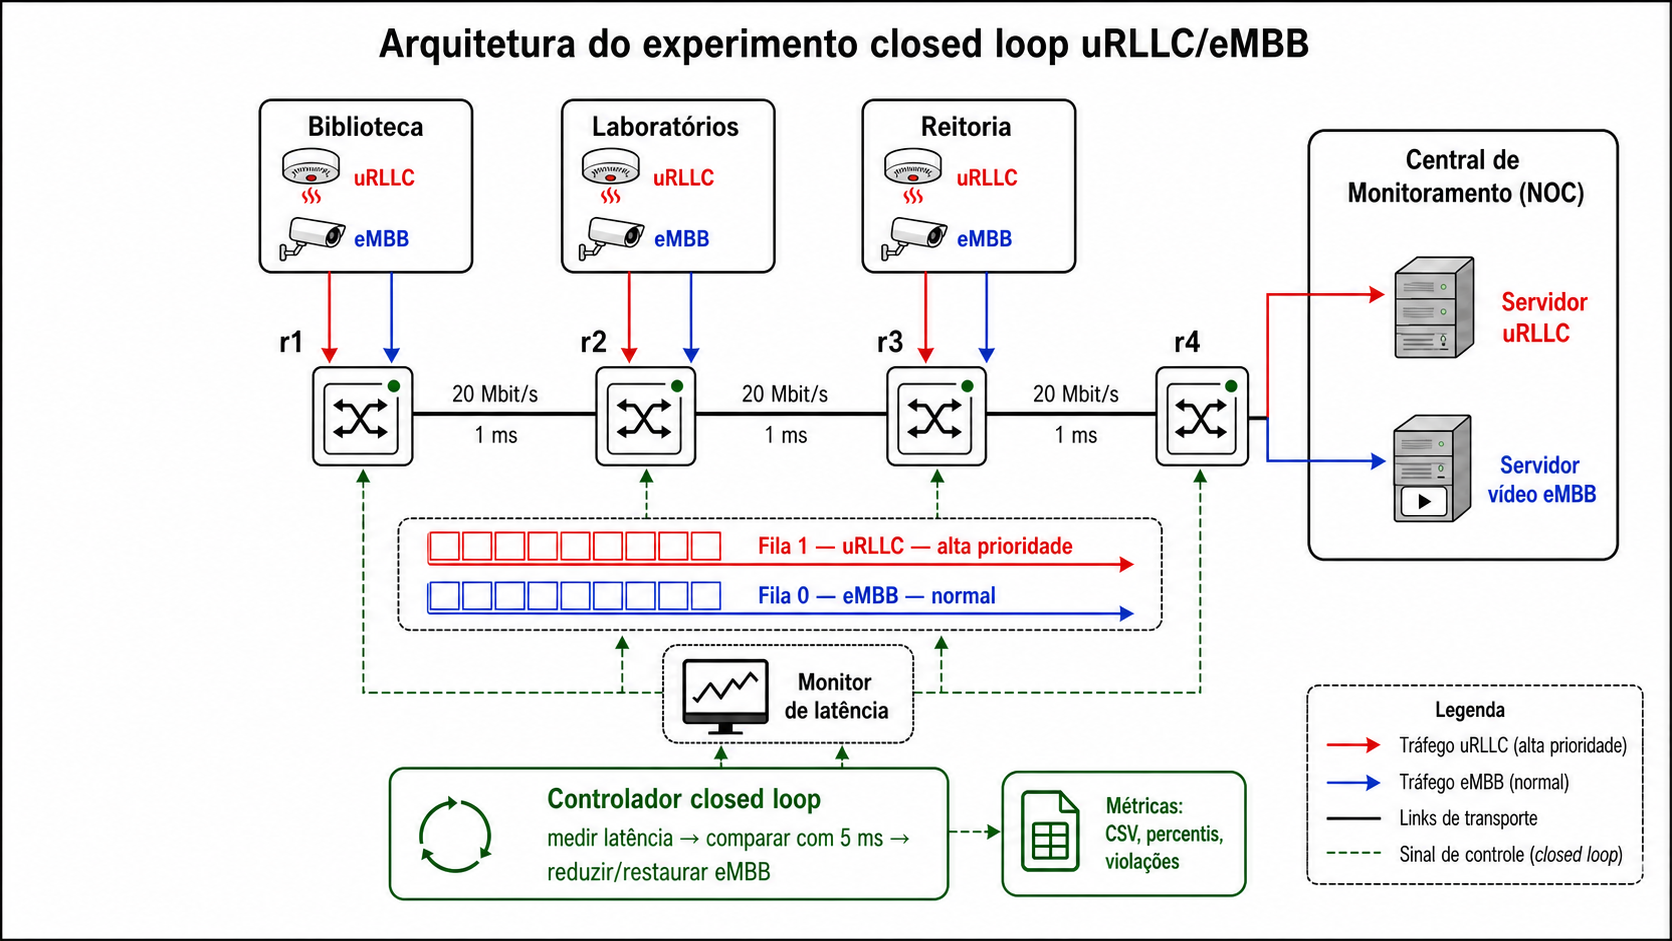
\includegraphics[width=\linewidth]{figuras/arquitetura_closed_loop.png}
			\caption{Arquitetura da rede 5G emulada, com três locais monitorados, quatro \textit{switches} Open vSwitch e a Central de Monitoramento.}
			\label{fig:arquitetura}
		\end{figure}

		A Figura~\ref{fig:arquitetura} mostra o caminho dos tráfegos de uRLLC e eMBB desde os sensores e câmeras até a central. Ela também evidencia que os três locais compartilham o mesmo meio de comunicação, dessa forma, é possível enxergar um cenário com possibilidades de congestionamento.
		
		% \subsection{Topologia e Bancada Experimental}
		
		% Descreva a topologia de rede criada no Mininet \cite{mininet}.
		% Os quatro n\'os de transporte foram implementados como switches
		% Open vSwitch (OVS) \cite{pfaff2015ovs}, configurados via OpenFlow 1.3
		% \cite{mckeown2008openflow} para encaminhamento L2 e prioriza\c{c}\~ao de
		% tr\'afego. Explique quantos hosts existem, quantos roteadores, como est\~ao
		% conectados e qual \'e o papel de cada n\'o. Especifique os
		% par\^ametros de cada enlace configurados com TCLink: largura de
		% banda, atraso e tamanho m\'aximo de fila. Justifique o limiar de
		% 5\,ms escolhido para o uRLLC com base no 5QI\,85 definido no
		% 3GPP TS\,23.501 \cite{3gpp23501}. Inclua uma figura da topologia
		% (\verb|\includegraphics|) com legenda descritiva. Ao final,
		% descreva o ambiente de testes: especifica\c{c}\~oes de hardware
		% (CPU, mem\'oria RAM), sistema operacional e vers\~oes de todas as
		% ferramentas usadas (Mininet, Python, Scapy, iperf3, Open vSwitch).
		
		% \subsection{Gera\c{c}\~ao de Tr\'afego}
		
		% Explique como cada tipo de tr\'afego foi gerado. Para o tr\'afego
		% uRLLC, descreva o script em Scapy \cite{scapy}: o tipo de pacote
		% (TCP SYN), a marca\c{c}\~ao DSCP EF com \texttt{tos=0xB8}
		% \cite{rfc3246}, a porta de destino e a taxa de envio. Apresente
		% a f\'ormula de c\'alculo da lat\^encia RTT por pacote:
		
		% \begin{equation}
		% 	\text{RTT}_i = (t_{\text{rx},i} - t_{\text{tx},i}) \times 10^3
		% 	\quad [\text{ms}]
		% \end{equation}
		
		% \noindent onde $t_{\text{tx}}$ \'e o instante de envio e
		% $t_{\text{rx}}$ \'e o instante de recep\c{c}\~ao registrados
		% pelo Scapy. Para o tr\'afego eMBB, descreva o uso do iperf3 \cite{iperf}
		% em modo UDP (ou TCP, quando indicado), com taxa
		% suficiente para saturar o enlace de gargalo e for\c{c}ar
		% viola\c{c}\~oes de lat\^encia.
		
		% \subsection{M\'etricas de Avalia\c{c}\~ao}
		
		% Defina cada m\'etrica que ser\'a usada na avalia\c{c}\~ao.
		% Apresente uma defini\c{c}\~ao clara e formal de cada uma, pois
		% o leitor precisa saber exatamente o que est\'a sendo medido.
		% As m\'etricas recomendadas s\~ao: taxa de viola\c{c}\~ao do
		% limiar (TV), que \'e a fra\c{c}\~ao de pacotes uRLLC com
		% RTT superior a 5\,ms; lat\^encia mediana (P50) e percentil 99
		% (P99), que descrevem a distribui\c{c}\~ao da lat\^encia; e
		% tempo de rea\c{c}\~ao (TR), definido como o intervalo entre
		% a primeira viola\c{c}\~ao detectada e o retorno da lat\^encia
		% abaixo do limiar ap\'os a atua\c{c}\~ao do sistema.
		
		% ===================================================================
		\section{Proposta}
		% ===================================================================
		
		A proposta desse projeto é desenvolver um sistema para prevenir incêndios. Desenvolvido em redes 5G, o sistema propõe utilizar sensores e câmeras para mitigar e prevenir possíveis incêndios usando tecnologia de comunicação ultraconfiável e de banda larga.

        \subsection{Ambientes de Monitoramento}
        
        Os ambientes que irão ser monitorados na simulação são a biblioteca, reitoria e laboratórios. Os sensores aplicados vão identificar a temperatura do ambiente, umidade, fumaça, chamas e gás. A câmera irá ativar o monitoramento assim que detectar algumas anomalias identificadas pelos sensores e que possam estar relacionadas a possíveis princípios de incêndio.

        Para os sensores, a tecnologia usada dentro do contexto das redes 5G, garantindo o mínimo de tempo possível de entrega para uma Central de Monitoramento, é o uRLLC (comunicação ultraconfiável e de baixa latência) \cite{3gpp23501,itu2017m2410}. Com essa aplicação, a comunicação deverá chegar com valor igual ou inferior a 5 milissegundos, dentro do contexto em que o projeto é proposto. O monitoramento com as câmeras também utilizará uma tecnologia de redes 5G, o eMBB (banda larga móvel aprimorada). Com essa aplicação, será possível enviar dados com uma carga maior de informação -- imagens -- que poderão gerar mais valor na identificação e solução dos elementos para prevenir incêndios no local.

        Os dispositivos de cada local estão conectados a quatro \textit{switches} em linha, em uma arquitetura simulada usando o Mininet, que emula a rede 5G. Um \textit{switch} fica responsável por conectar os servidores de monitoramento de sensores e de câmeras, cada um processando dados de forma que não sobrecarregue ou gere perdas de dados na comunicação.
        
        \subsection{Tráfegos uRLLC e eMBB}
        
        As mensagens da rede uRLLC passam pela porta TCP 5000, enquanto o fluxo relacionado ao vídeo eMBB é gerado pelo iperf3 através das portas 5001--5003. Essas configurações são utilizadas para validar os resultados e os objetivos da proposta. Um mecanismo importante nessa construção é a Qualidade de Serviço (QoS) adaptativa \cite{olegario2024qos5g}, que cria filas: a fila 1 representa o tráfego uRLLC e a fila 0 representa o eMBB. Essas regras são implementadas por meio do OpenFlow \cite{mckeown2008openflow} nos \textit{switches} OVS \cite{pfaff2015ovs}. A fila uRLLC tem banda reservada, enquanto a banda do eMBB é ajustável, pois esse tráfego não possui a mesma prioridade.

        \subsection{\textit{Closed loop} e Ajustes de Latência}
        
        Para assegurar o monitoramento, é utilizado o \textit{closed loop} \cite{simao2025mecanismo}. O ciclo segue a seguinte sequência: a central observa cada mensagem uRLLC e mede a latência; o controlador verifica o limite de 5 ms e, se esse limite for ultrapassado, reduz a taxa máxima das filas eMBB de 20 para 2 Mbit/s \cite{linuxhtb}, aliviando a rede para o uRLLC. Todo esse processo é repetido e verificado pelo \textit{closed loop} para manter uma rede estável, principalmente para os sensores.

        No caso de o tráfego eMBB ser limitado ou ajustado para priorizar o tráfego uRLLC, o tráfego das câmeras não é interrompido e a rede permanece ativa. O monitor não ajusta as prioridades somente com base na primeira latência acima de 5 ms. Para ativar e realizar os ajustes, é utilizado um método chamado histerese: se houver latências acima de 5 ms duas vezes consecutivas, a proteção será ativada; quando a latência voltar ao normal, serão aguardadas três medições sequenciais abaixo de 5 ms para desativá-la.
        
		
	
		% ===================================================================
		\section{Avalia\c{c}\~ao}
		% ===================================================================
		
		O projeto seguiu alguns pilares para demonstrar os resultados produzidos para a avaliação, que são quatro cenários: Isolado; Sem QoS; QoS Estático; e \textit{closed loop}.
		
		\subsection{Configura\c{c}\~ao Experimental}

        O ambiente dos experimentos é todo virtualizado, desde os \textit{switches} até os sensores. Tudo é executado dentro do Docker, usando Linux e rodando no macOS. Foram realizados cinco testes para cada um dos quatro cenários, totalizando uma bateria de 20 testes.

        \subsection{Resultados e Discussões}
        
        O primeiro cenário testado foi o isolado. Nele, apenas o tráfego uRLLC está ativo, sem concorrer com o eMBB; somente os sensores transmitem dados para a central. Com isso, a latência se mostrou abaixo de 5 ms em todos os casos. A tabela de conformidade e a CDF apresentam melhor os resultados do cenário isolado.

		\begin{table}[ht]
			\centering
			\caption{Métricas agregadas de conformidade do tráfego uRLLC.}
			\label{tab:conformidade-urllc}
			\scriptsize
			\resizebox{\columnwidth}{!}{%
				\begin{tabular}{lrrrrr}
					\toprule
					Cenário & Tentativas & Falhas & Violações & Perdas (\%) & Não conformes (\%) \\
					\midrule
					Isolado & 8838 & 0 & 7 & 0,00 & 0,08 \\
					Sem QoS & 1124 & 148 & 364 & 13,17 & 45,55 \\
					QoS estático & 887 & 129 & 318 & 14,54 & 50,39 \\
					\textit{Closed loop} & 533 & 158 & 9 & 29,64 & 31,33 \\
					\bottomrule
				\end{tabular}%
			}
		\end{table}

		\begin{figure}[ht]
			\centering
			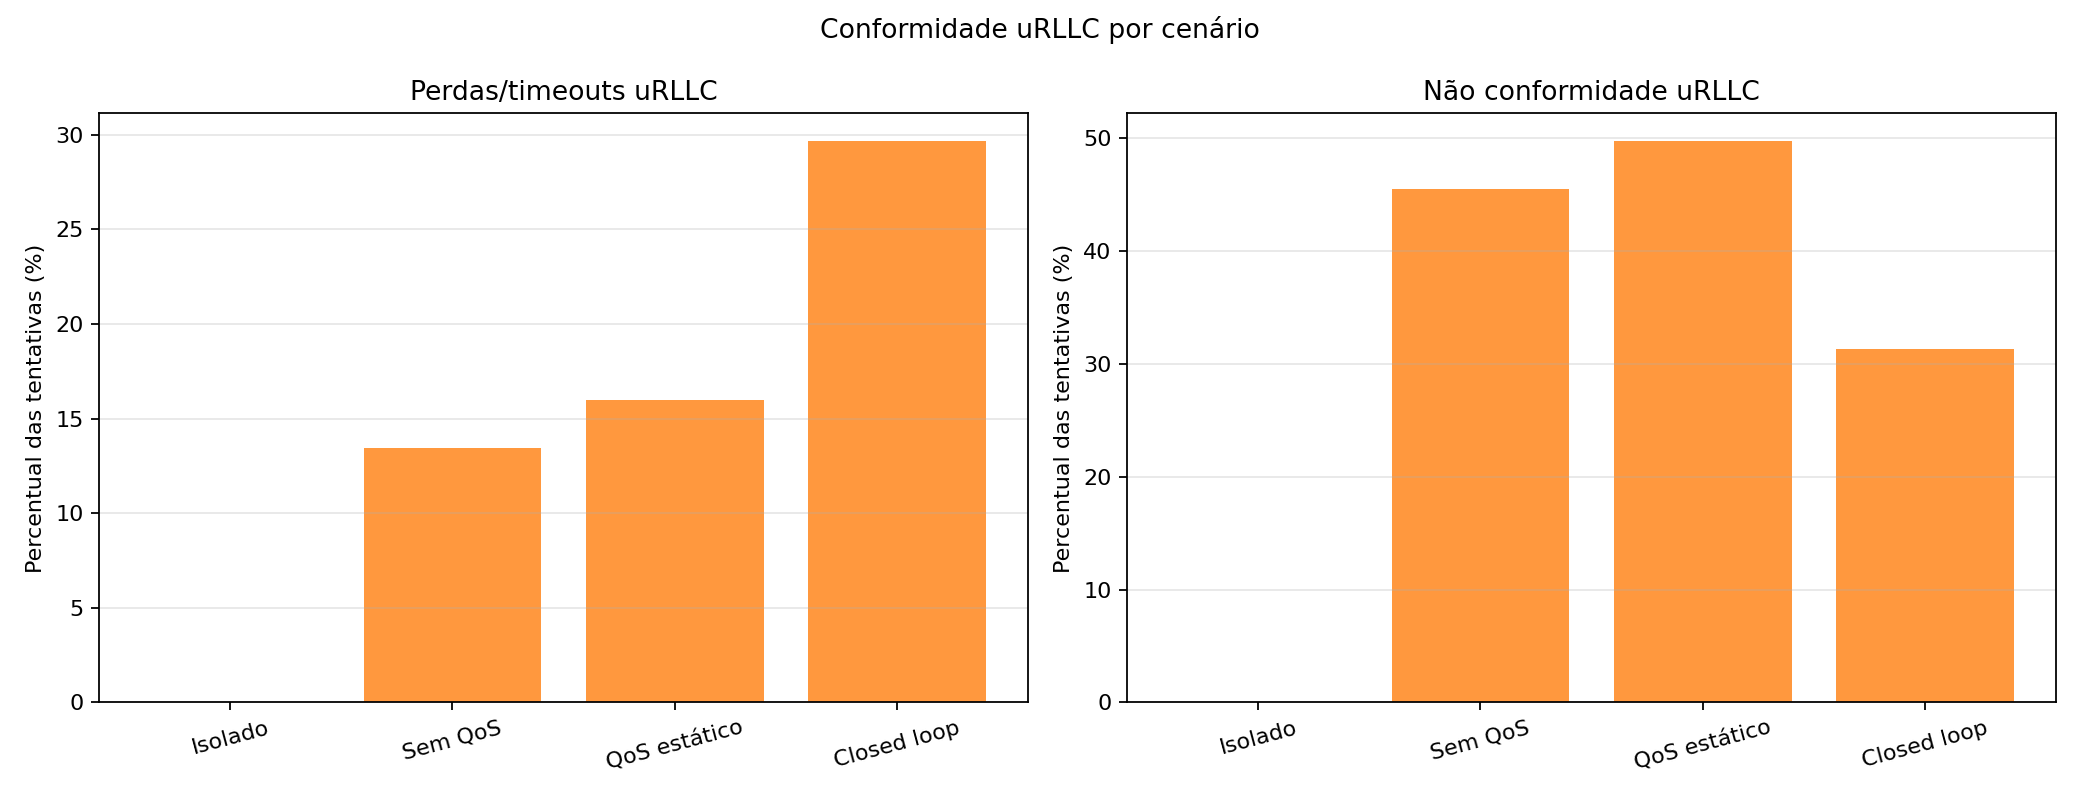
\includegraphics[width=\linewidth]{figuras/metricas_urllc.png}
			\caption{Perdas, \textit{timeouts} e não conformidade efetiva do tráfego uRLLC por cenário.}
			\label{fig:metricas-urllc}
		\end{figure}

		A Figura~\ref{fig:metricas-urllc} e a Tabela~\ref{tab:conformidade-urllc} mostram que a análise deve considerar todas as tentativas, incluindo perdas e \textit{timeouts}. Com essa métrica, o \textit{closed loop} melhora o resultado em relação aos cenários concorrentes, mas ainda não garante o limite de 5 ms.

		\begin{figure}[ht]
			\centering
			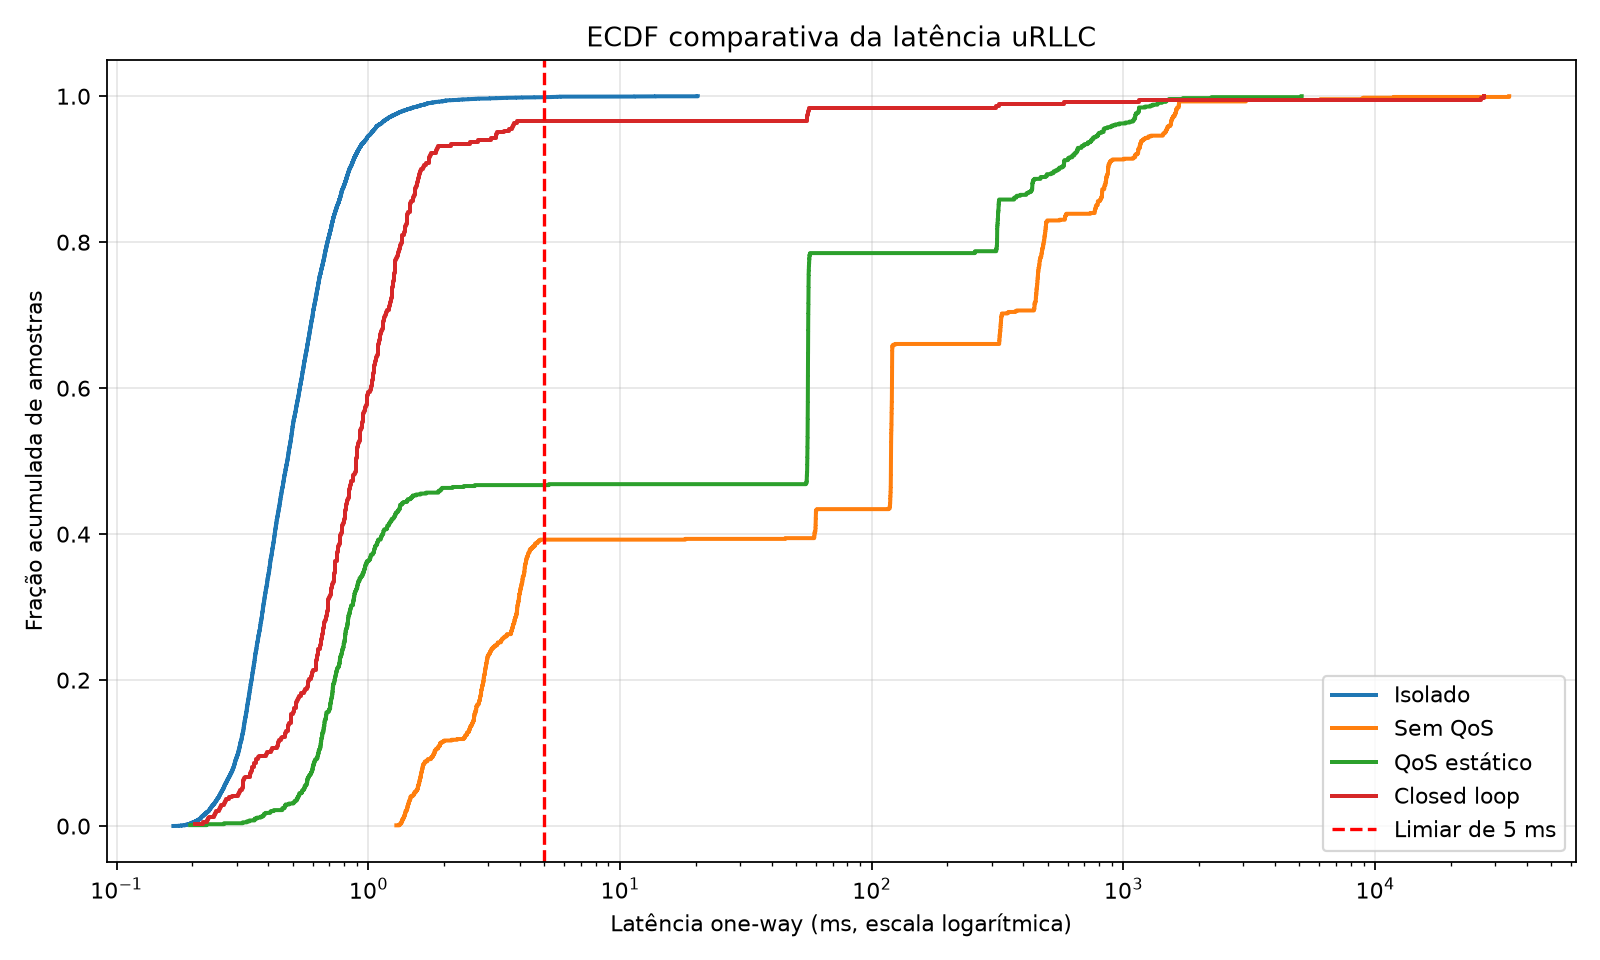
\includegraphics[width=\linewidth]{figuras/comparacao_cdf.png}
			\caption{Função de distribuição acumulada da latência uRLLC nos quatro cenários avaliados.}
			\label{fig:cdf-urllc}
		\end{figure}

		Na Figura~\ref{fig:cdf-urllc}, a linha tracejada na vertical de cor vermelha representa o limite de 5 ms. A comparação deve destacar a posição de cada curva em relação a esse limite e esclarecer que a CDF considera apenas amostras recebidas, não substituindo a métrica de não conformidade efetiva.

        No cenário sem QoS, o tráfego fica sem classificação de prioridade, afetando o desempenho da rede. Como é possível observar na figura de conformidade de tráfego, a não conformidade foi de 45,55\%, com p95 de 1455,314 ms. No cenário com QoS estático, o tráfego uRLLC é colocado em uma fila de prioridade durante toda a execução; nesse caso, a configuração da rede não é alterada independentemente de suas condições. Ainda considerando a análise estatística, o p95 apresentou um valor alto, de 804,040 ms, devido a perdas e \textit{timeouts} na comunicação. Houve uma melhora, mas não suficiente para garantir o limite de 5 ms.

		\begin{table}[ht]
			\centering
			\caption{Estatísticas de latência uRLLC; percentis calculados sobre amostras recebidas.}
			\label{tab:latencia-urllc}
			\scriptsize
			\resizebox{\columnwidth}{!}{%
				\begin{tabular}{lrrrr}
					\toprule
					Cenário & Mediana (ms) & p95 (ms) & p99 (ms) & $>5$ ms (\%) \\
					\midrule
					Isolado & 0,476 & 1,029 & 1,707 & 0,14 \\
					Sem QoS & 119,291 & 1455,314 & 1663,662 & 60,75 \\
					QoS estático & 55,466 & 804,040 & 1367,169 & 53,28 \\
					\textit{Closed loop} & 0,896 & 3,233 & 367,283 & 3,39 \\
					\bottomrule
				\end{tabular}%
			}
		\end{table}

		A Tabela~\ref{tab:latencia-urllc} permite separar a melhoria da distribuição de latência do efeito das perdas. O QoS estático reduz os percentis em relação ao cenário sem QoS, mas o percentual de não conformidade efetiva permanece elevado porque os \textit{timeouts} também são contabilizados.

        O último cenário dos testes foi o \textit{closed loop}, que é o foco da proposta do projeto. Aqui, o controlador monitora constantemente a latência uRLLC. Após duas violações consecutivas do limite de 5 ms, a taxa máxima da fila eMBB é reduzida de 20 para 2 Mbit/s. Quando são obtidas três medições seguidas abaixo ou iguais a 5 ms, o controlador restaura a taxa do eMBB. A não conformidade efetiva foi reduzida para 31,33\%. O p95 apresentou valor de 3,233 ms entre os dados recebidos. O \textit{closed loop} trouxe melhorias, mas apresentou 29,64\% de perdas ou \textit{timeouts}. A vazão do eMBB caiu para 0,932 Mbit/s, com perda de 92,27\% nesses testes. O mecanismo protegeu o tráfego uRLLC, mas com o custo de desfavorecer o serviço eMBB.

		\begin{table}[ht]
			\centering
			\caption{Vazão recebida e perdas do tráfego eMBB sob concorrência com uRLLC.}
			\label{tab:vazao-embb}
			\scriptsize
			\begin{tabular}{lrr}
				\toprule
				Cenário & Vazão (Mbit/s) & Perda (\%) \\
				\midrule
				Sem QoS & 6,469 & 46,00 \\
				QoS estático & 5,766 & 51,87 \\
				\textit{Closed loop} & 0,932 & 92,27 \\
				\bottomrule
			\end{tabular}
		\end{table}

		\begin{figure}[ht]
			\centering
			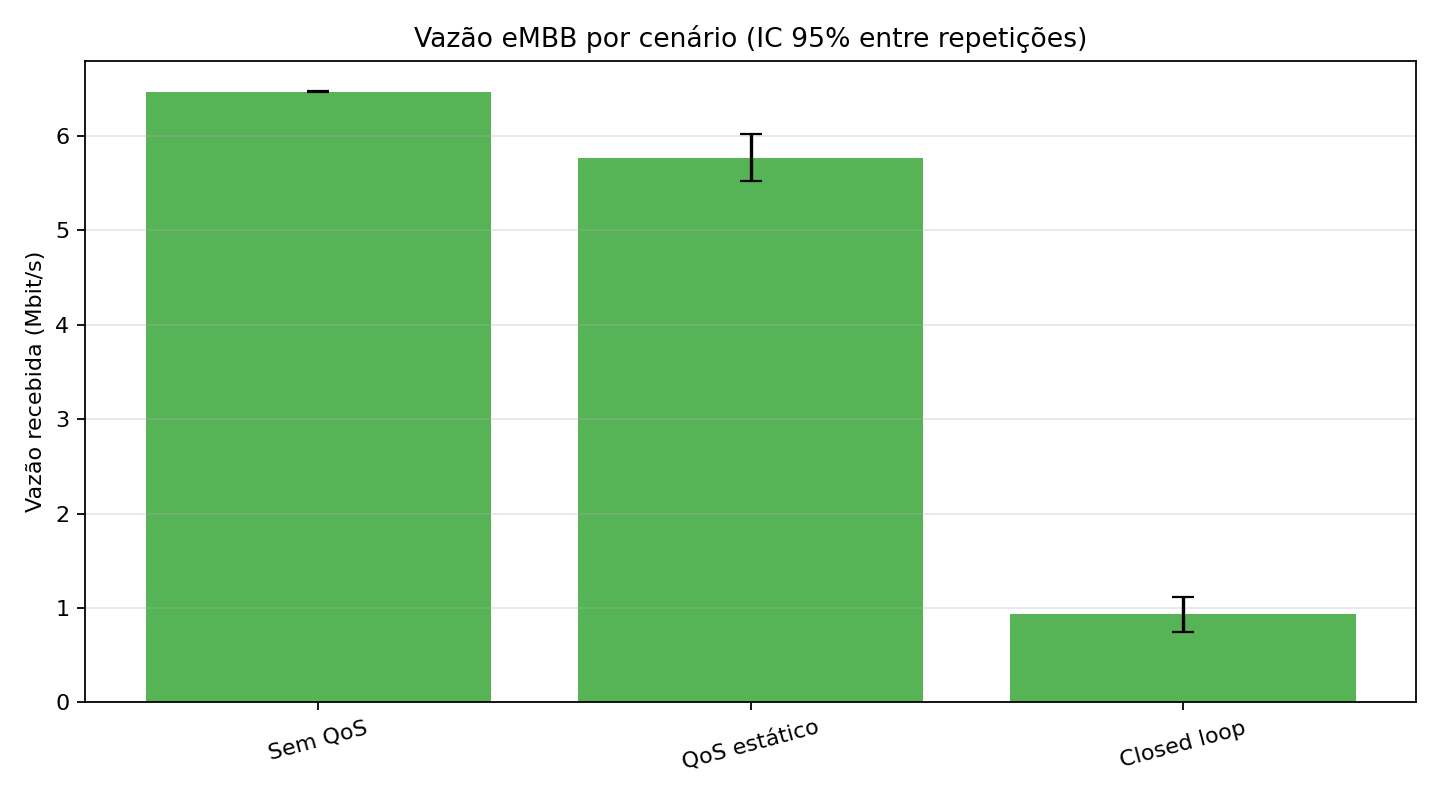
\includegraphics[width=\linewidth]{figuras/vazao_embb.png}
			\caption{Vazão eMBB recebida por cenário, com intervalo de confiança de 95\% entre as repetições.}
			\label{fig:vazao-embb}
		\end{figure}


		\FloatBarrier
		
		
		
		% ===================================================================
		\section{Conclus\~oes}
		% ===================================================================

		Este trabalho apresentou um sistema de monitoramento e prevenção de incêndios em um cenário de rede 5G emulada. A proposta utiliza sensores para gerar tráfego uRLLC e câmeras para gerar tráfego eMBB, conectados por quatro \textit{switches} Open vSwitch e monitorados por uma Central de Monitoramento. O controle da rede foi implementado com filas QoS e um controlador \textit{closed loop} capaz de ajustar a taxa do tráfego eMBB de acordo com a latência observada no tráfego uRLLC.

		A avaliação foi realizada com quatro cenários e cinco repetições de 60 segundos para cada cenário. A não conformidade efetiva foi de 0,08\% no cenário isolado, 45,55\% no cenário sem QoS, 50,39\% no QoS estático e 31,33\% no \textit{closed loop}. Entre os pacotes recebidos, o \textit{closed loop} apresentou p95 de 3,233 ms; entretanto, ainda foram observados 29,64\% de perdas ou \textit{timeouts}. Portanto, a redução da não conformidade não representa uma garantia de que todas as tentativas atenderam ao limite de 5 ms.

		Os resultados também mostraram um compromisso entre a proteção do uRLLC e o desempenho eMBB. No \textit{closed loop}, a vazão eMBB foi reduzida para 0,932 Mbit/s, com 92,27\% de perdas. Assim, o mecanismo demonstrou capacidade de reduzir a latência dos pacotes uRLLC recebidos sob concorrência, mas ainda precisa ser interpretado como uma estratégia de proteção parcial, cujo custo sobre o tráfego eMBB deve ser considerado. Como os experimentos foram realizados em ambiente emulado, os resultados caracterizam as condições avaliadas no laboratório e não constituem garantia de desempenho em uma rede 5G real.
		
		% As conclus\~oes encerram o artigo de forma objetiva. N\~ao
		% apresente resultados novos aqui -- apenas consolide o que j\'a
		% foi dito nas se\c{c}\~oes anteriores. Escreva tr\^es par\'agrafos.
		
		% O \textbf{primeiro par\'agrafo} faz a s\'intese do trabalho:
		% retome o problema abordado, a proposta apresentada e o principal
		% resultado obtido. Seja direto e use n\'umeros concretos dos seus
		% experimentos. Exemplo de estrutura: ``Este artigo apresentou um
		% sistema de \textit{closed loop} para controle de lat\^encia de
		% fluxos uRLLC na rede de transporte 5G, utilizando Open vSwitch
		% com QoS/OpenFlow. Os resultados demonstraram que a abordagem
		% reduziu as viola\c{c}\~oes do limiar de 5\,ms, mantendo a
		% lat\^encia m\'edia abaixo de 2,5\,ms mesmo na presen\c{c}a de
		% tr\'afego eMBB.''
		
		% O \textbf{segundo par\'agrafo} confirma as contribui\c{c}\~oes:
		% retome cada item listado na Introdu\c{c}\~ao e afirme que foi
		% alcan\c{c}ado, fazendo refer\^encia \`a se\c{c}\~ao ou resultado
		% que comprova isso.
		
		% O \textbf{terceiro par\'agrafo} aponta os trabalhos futuros:
		% direcoes concretas que voc\^e ainda n\~ao fez mas que seriam
		% poss\'iveis extens\~oes naturais do trabalho. Exemplos:
		% valida\c{c}\~ao em hardware real com switches Intel Tofino,
		% extens\~ao para cen\'arios de federa\c{c}\~ao multi-dom\'inio
		% usando VXLAN como substrato, ou incorpora\c{c}\~ao de
		% classifica\c{c}\~ao de dispositivos com aprendizado de m\'aquina
		% diretamente no plano de dados.
		
		% ===================================================================
		\bibliographystyle{sbc}
		\bibliography{referencias}
		
	\end{document}
